\chapter{Численная модель стримерно-лидерной стадии молнии}
\label{sec:model-intro}
Моделирование процесса молнии является сложной задачей, характеризующейся большим диапазоном пространственных и временных масштабов процессов, большим количеством эволюционирующих компонент и сложной геометрией, обладающей фрактальной структурой. В силу этих факторов, применимость аналитических методов к данной задаче ограничена, и наиболее перспективным является численное моделирование.

Актуальные подходы к моделированию молнии можно разделить на несколько категорий:
\begin{enumerate}
	\item \textbf{Плазмохимические модели.} Расчитывается стационарная, либо нестационарная кинетика молниевого канала на различных стадиях. Учитываются десятки и сотни плазмохимических реакций. Модели применимы к широкому спектру разрядов, например "--- к моделированию т.\,н. эльфов и спрайтов \cite{Sentman2008}\cite{Kossiy1994}. Однако такие модели вычислительно сложны, и вследствие этого либо нуль-мерны, либо <<1,5-мерны>> "--- предполагают аксиально-симметричную форму канала разряда. Такой подход не позволяет воспроизводить сложную геометрии молниевого разряда. Строго говоря, плазмохимические модели воспроизводят пробой в воздухе, но ещё не молнию.
	\item \textbf{Электродинамические модели.} Описывается изменение распределения зарядов и токов в молниевом канале. Такие модели исключают влияние электрических процессов на геометрию разряда и чаще всего применяются для описания главной стадии молнии. Для воспроизведения процесса инициации молнии их применимость ограничена. 
	\item \textbf{Дискретные модели, клеточные автоматы.} Воспроизводят динамику молниевого канала на этапе его формирования на дискретной сетке. Ячейки сетки могут находиться в состоянии проводимости и быть частью канала. Каждой ячейке соответствует набор динамических переменных, которые эволюционируют во времени. Дискретные модели воспроизводят сложную геометрию молнии, однако имеют строгие ограничения по масштабу и разветвлённости элементов молнии. В силу того, что данные модели являются высокоуровневыми, они требуют параметризаций процессов, происходящих в ячейках расчётной сетки. Выбор параметризации является сложной задачей. Существующие дискретные модели молнии описывают распространение лидера и не рассматривают процесс его возникновения, \textit{стримерно-лидерный переход.} Примерами дискретных моделей служат работы \cite{Iudin2017}
\end{enumerate}

Одним из наиболее важных и неисследованных этапов развития молнии является процесс её инициации \cite{Dwyer2014}. На данный момент не существует единой точки зрения на то, как достаточно длинный для поддержания собственного развития хорошо проводящий лидерный канал формируется в грозовом облаке, максимальная напряженность электрического поля в котором на порядок ниже поля пробоя воздуха \cite{Marshall1995}. Предпринятые многочисленными исследователями попытки решения данной проблемы вылились в набор конкурирующих гипотез, каждая из которых столкнулась с определенными трудностями.

Первый механизм восходит к работам \cite{Loeb1966, Phelps1974, Griffiths1976}, в которых изучалась возможность инициации стримеров с гидрометеоров. Предполагается, что положительный стример зарождается в области усиленного поля, возникающего при поляризации одиночного гидрометеора во внешнем поле или при сближении пары противоположно заряженных гидрометеоров. При этом считается, что развивающаяся с гидрометеора система положительных стримеров или несколько перекрывающихся стримерных систем, развивающихся с соседних гидрометеоров, выносят положительный заряд в направлении роста и аккумулируют отрицательный заряд в точке старта, что, в конце концов, приводит к появлению пучка отрицательных стримеров, растущих в противоположном направлении \cite{Griffiths1976}. Прогреваясь токами поляризации, биполярная стримерная система формирует внутри себя горячий лидерный канал, способный к самостоятельному поддержанию своего дальнейшего распространения. Недостаток данного механизма состоит в том, что для обеспечения устойчивого развития стримерной системы необходимо наличие либо области с электрическим полем, превосходящим максимально наблюдаемые облачные поля \cite{Griffiths1976}, либо гидрометеора с аномально большим аспектным отношением \cite{Dubinova2015}. В моделях, посвященных инициации положительного стримера с гидрометеора (см., например, \cite{Sadighi2015, Cai2017}), указывается также на необходимость предварительной ионизации, источник которой, как правило, не уточняется.

Вторая гипотеза основана на предложенном Гуревичем \cite{Gurevich1992} механизме пробоя на высокоэнергичных убегающих электронах, для которых эффективная сила трения убывает в интервале от 0.1\,кэВ до 1\,МэВ. В данном энергетическом диапазоне электрон может набирать энергию вплоть до 1\,МэВ, при которой сила трения становится достаточной для компенсации ускоряющего действия электрического поля. При удачном месте возникновения первых затравочных убегающих электронов, появляющихся под действием ионизации нейтралов частицами космических лучей, они могут породить электронную лавину, что, в свою очередь, способно привести к электрическому пробою облачной среды. Предполагается, что пробой на убегающих электронах способен создать плазменное пятно, поляризация на границах которого приводит к существенному усилению поля \cite{Gurevich1999}. Если плазма, поляризуясь, локально приобретает форму стримерной головки, запускается описанный выше стримерный механизм формирования лидера молнии \cite{Gurevich1999}. Несмотря на то, что пробой на убегающих электронах требует полей, примерно равных максимальным измеренным в грозовом облаке значениям, необходимая для реализации данного процесса протяженность области сильного поля достигает километра \cite{Gurevich2001}, что противоречит данным наблюдений.

В своей работе \cite{Dwyer2005} Двайер оспаривает возможность данного сценария, указывая на то, что затравочные электроны, произведенные частицами космического ветра, должны иметь большой поперечный разброс, вследствие чего производимая ими плазма будет сильно разреженной. Вместе с тем, Двайер предлагает позитронную модернизацию механизма пробоя на убегающих электронах, в которой развитие разряда поддерживается петлей положительной обратной связи между позитронными и гамма лучами и может привести к возникновению локальной зоны сильного электрического поля вблизи границы распространения разрядной активности, даже несмотря на отсутствие достаточно сильного крупномасштабного электрического поля, необходимого для механизма, предложенного Гуревичем. Проведенные Двайером вычисления показывают, что за счет данного механизма электрическое поле даже в относительно компактной области может достичь значений, превышающих 1\,МВ/м при давлении на уровне моря и, таким образом, поддержать процесс <<традиционного>> пробоя, приводящего к инициации молнии.

Еще один гибридный механизм, соединяющий идею пробоя на убегающих электронах с инициацией положительных стримерных систем с поверхности гидрометеоров, был предложен Петерсеном \cite{Petersen2008}. В рамках данной модели пробой на убегающих электронах обеспечивает наличие предварительной ионизации, необходимой для инициации положительных стримеров с поляризованных локальным полем гидрометеоров. Возникающий пучок положительных стримеров по мере развития накапливает отрицательный заряд в точке своего основания, локально усиливая поле и создавая условия для возникновения противоположно направленных отрицательных стримеров. Менее многочисленные, но более мощные отрицательные стримеры теперь уже биполярной стримерной системы, прогреваясь, формируют канал пространственного лидера и, участвуя в процессе разделения заряда, усиливают поле на периферии разрядной структуры, провоцируя появление еще одной (вторичной) системы положительных стримеров, развитие которой происходит подобным же образом. Далее вторичная стримерная система поляризуется по аналогии с исходной. В ходе совместного развития положительные стримеры вторичной системы сливаются с отрицательными стримерами первичной, создавая единый канал, прогреваемый токами выравнивания потенциала. В результате многократного повторения данного процесса перекрывающаяся и сливающаяся цепочка биполярных стримерных систем формирует канал лидера молнии.

%Дмитрий Игоревич просил убрать этот абзац из введения
%Ризон \cite{Rison2016}, основываясь на многочисленных натурных измерениях, предполагает, что молниевый разряд может инициироваться так называемым быстрым пробоем на положительных стримеров (fast positive breakdown). Полевые измерения, однако, показывают, что появление молний не всегда сопровождается излучением, характерным для данного типа разряда.

Недавно в работе \cite{Iudin2017} был предложен принципиально новый механизм инициации молнии, основанный на индуцированном шумом кинетическом переходе, происходящем в стохастическом поле заряженных гидрометеоров. Результатом неравновесного фазового перехода являются пятна ионной плазмы с линейными размерами, достигающими нескольких дециметров, и временем жизни порядка нескольких десятков миллисекунд (см. также \cite{todo}). При этом в работе \cite{Iudin2017} подчеркивается, что резкий рост ионной проводимости происходит в экспоненциально редких компактных областях пространства на фоне исчезающе малых изменений средней проводимости среды. В ходе поляризации, обусловленной крупномасштабным электрическим полем грозы, поле на концах плазменных пятен усиливается до величины, достаточной для инициации положительных стримеров. По мере роста концентрации пятен ионной плазмы, коллективная динамика положительных стримерных систем обеспечивает появление лидерного канала в соответствие с качественной картиной описанных выше сценариев Леба и Петерсона, основанных на традиционной доктрине электрического пробоя в атмосфере.

Построение количественной модели зарождения молниевого разряда, основанной на предложенном в работе \cite{Iudin2017} механизме инициации положительных стримеров с поляризованных ионных областей, обладающих повышенной проводимостью, составляет содержание данной главы. Настоящая работа является инновационным развитием модельного подхода \cite{IudinRakov2017}, в котором изложены базовые принципы стохастического развития древа молниевого разряда как саморазвивающегося направленного динамического графа с нелинейными связями. В данной работе решен целый ряд актуальных для моделей развития молниевых разрядов проблем. Во-первых, в предложенной модели впервые отсутствует привязка вершин проводящих связей к узлам пространственной решетки, то есть направление роста разрядного канала не имеет принципиальных ограничений, свойственных всем остальным подобным моделям, в которых морфология разрядных структур ограничена шагом пространственной решетки. Такой подход не ограничивает ни минимальное расстояние между близко расположенными разрядными каналами, ни число связей, растущих из одной вершины. Во-вторых, в настоящей модели впервые последовательно учитывается асимметрия полей развития положительных и отрицательных стримеров. В-третьих, в модели реализован самосогласованный механизм стримерно-лидерного перехода, происходящего посредством развития протекающей в пучке стримерных каналов ионизационно-перегревной неустойчивости. Данные свойства модели позволили успешно воспроизвести основные особенности коллективной динамики множества одновременно развивающихся стримерных разрядов, которая, как это следует из результатов моделирования, является принципиальной основой формирования билидерного канала молниевого лидера в грозовом облаке.

\section{Постановка задачи}
\label{sec:model-base}
В данной работе моделируется развитие молниевого разряда в области однородного крупномасштабного электрического поля грозы с размерами порядка сотен метров. Предполагается, что область пространства, в которой начинает развиваться разрядное дерево, находится на высоте 6~км над уровнем моря, что характерно для исходной точки развития молниевого разряда типа облако-земля \cite{Rison2016}. Напряженность однородного вертикально ориентированного электрического поля $\vec E_{ext}$, в котором формируется разряд, составляет~$2,7 \text{кВ}/\text{см}$, что соответствует максимальному измеренному в грозовом облаке значению \cite{Marshall1995}. В связи со значительной удаленностью разрядного древа от поверхности земли (максимальное расстояние между отдельными узлами разряда много меньше расстояния до земли) в данной модели расчет электрического поля происходит без учёта отраженного в ней заряда. В целях оптимизации расчетов моделирование происходит с автоматическим выбором шага по времени. Характерный временной шаг составляет $10^{-11} - 10^{-9}$~c.

Электрическая цепь, образуемая проводящими структурами молниевого разряда, моделируется в виде динамического графа, вложенного в трехмерное пространство. Базовыми элементами модели являются вершины и рёбра графа. Вершины соответствуют ёмкостным элементам цепи, а рёбра~"--- резистивным. Пример фрагмента такого графа представлен на рис.~\ref{fig:net-frag}. 

В отношении разработанной модели применяется термит <<транспортная самоорганизующаяся модель>> (ТСМ) "--- способ моделирования физических систем, в которых происходит перенос динамических переменных в пространстве в соответствии с геометрией, определяемой этими динамическими переменными.

В процессе инициации молнии возникает сложная система стримеров и развивается лидер. 
Эти объекты образуют разветвлённую электрическую цепь, которую можно представить в виде графа, вложенного в трёхмерное пространство, структура которого меняется с течением времени. Пример фрагмента такого графа представлен на \figRef{fig:net-frag}. Вершинам и рёбрам графа сопоставляются определённые параметры и динамические переменные. По мере совершенствования модели набор динамических переменных и параметров может дополняться и изменяться.

\begin{figure}[h]
	\center{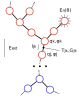
\includegraphics[width=0.5\linewidth]{net-frag.pdf}}
	\caption{Молниевый разряд в виде графа}
	\label{fig:net-frag}
\end{figure}

Каждой вершине графа с индексом $i$ соответствует динамическая переменная $q_i$~"--- сосредоточенный в ней электрический заряд. Каждому ребру с индексом $j$ ставится в соответствие удельная проводимость~$G_j$ и температура нейтрального газа~$T_j$, которые также являются динамическими переменными задачи. Параметром вершины является её эффективный радиус~$R=3\,\text{см}$. Все рёбра представляют собой цилиндры и имеют одинаковые длины~$l=30\,\text{см}$ и радиусы $r=1,4\text{мм}$. Таким образом, с точки зрения электродинамики, система представляет собой совокупность идеально проводящих сфер, соединенных проводниками с конечными проводимостями, благодаря чему модель учитывает распределенную ёмкость проводников. Индуктивности каждой отдельной связи и образуемых ими электрических цепей считаются пренебрежимо малыми.

Эволюция системы определяется двумя процессами: изменением динамических переменных, соответствующих вершинам и рёбрам, а также бифуркациями, изменяющими структуру графа. Первый процесс моделирует перераспределение заряда, нагрев, остывание и изменение проводимости различных частей системы, а второй~"--- пространственное развитие разряда.

\subsection{Эволюция динамических переменных}
Электрическое поле в любой точке пространства с радиус-вектором $\vec r$ находится в электростатическом приближении и вычисляется следующим образом:
\begin{equation}
	\begin{gathered}
		\varphi(\vec{r}) = \kelec \sum_{i=1}^{N} \frac{q_i}{|\vec{r}-\vec{r}_i|} + \varphi_{ext} (\vec{r}) \\
		\vec{E}(\vec{r}) = \kelec \sum_{i=1}^{N} \frac{q_i (\vec{r}-\vec{r}_i)} {|\vec{r}-\vec{r}_i|^3} + \nabla \varphi_{ext}(\vec{r})
	\end{gathered}
	\label{eq:coulomb}
\end{equation}
где $N$ "--- количество вершин графа, $r_i$ и $q_i$ "--- координаты и заряд вершины с индексом~$i$, $\varphi_{ext} (\vec{r})$ "--- потенциал, создаваемый внешним электрическим полем $\vec E_{ext}$. Потенциал вершины~$i$, представляющей собой идеально проводящую сферу радиуса $R$, можно представить как
\begin{equation}
	\begin{gathered}
		\varphi_i = \kelec \sum_{j \ne i} \frac{q_j}{|\vec{r}_k-\vec{r}_j|} + \kelec \frac{q_i}{R} + \varphi_{ext} (\vec{r}).
	\end{gathered}
\end{equation}

Эволюция заряда вершины~$i$ описывается уравнением непрерывности
\begin{equation}
	\dot q_i = \sum_{j=1}^{N_i} I_j,
\end{equation}
где $N_i$ "--- кратность вершины $i$, а $I_j$ "--- ориентированные токи, втекающие в вершину $i$ или вытекающие из нее по примыкающим к данной вершине рёбрам. Ток, текущий по ребру $j$, определяется его проводимостью и разностью потенциалов на его концах:
\begin{equation}
	I_j = G \frac{\pi r^2}{L}(\varphi_{j1} - \varphi_{j2})
\end{equation}
где $r$ и $L$ "--- радиус и длина ребра, $\varphi_{j1}$ и $\varphi_{j2}$ "--- потенциалы соединяемых ребром вершин.

В процессе развития разряда происходит увеличение температуры сосредоточенного в нем нейтрального газа. Когда температура канала превышает характерный порог $T^* = 3000\,K$, развивается ионизационно-перегревная неустойчивость. Эволюцию температуры нейтрального газа в объёма ребра $k$ можно описать как:
\begin{equation}
	\frac{dT_k}{dt} = \frac{1}{\pi L_k R_k^2 \rho c } I_k (\varphi_{k1} - \varphi_{k2})
	\label{eq:temp-evo}
\end{equation}
где $c=1\,\text{кДж}/(\text{кг}\cdot\text{К})$ "--- удельная теплоёмкость воздуха, $\rho=0,63\,\text{кг}/\text{м}^3$ "--- его плотность. Выражение~\eqref{eq:temp-evo} описывает джоулев нагрев газа в приближении отсутствия потери тепла за счёт теплового потока с поверхности канала. Это допустимо, так как процесс теплопередачи в воздухе на масштабах порядка радиуса канала происходит существенно дольше, чем развитие модельного разряда ($1\-2$\,мс).

Эволюция проводимости ребра $k$ и параметризация развития ионизационно-перегревной неустойчивости описывается следующим образом:

\begin{equation}
	G_k = [1-\alpha(T_k)] G_k^I + \alpha(T_k) G_k^{II}
	\label{eq:ioi-param}
\end{equation}
\begin{equation}
	\frac{dG_k^I}{dt} = \left[ \eta \left( \frac{\varphi_{k1} - \varphi_{k2}}{L_k}\right)^2 - \beta \right]G_k^I
	\label{eq:cond-no-ioi}
\end{equation}
где $G_k^I$ и $G_k^{II}$ "--- характерные проводимости канала до и после развития неустойчивости соответственно, $\alpha(T)$ "--- сглаженная степ-функция, описывающая скачкообразный переход от стримерной проводимости к лидерной, происходящий при приближении температуры канала к пороговому значения $T^* = 3000\,K$:
\begin{equation}
	\alpha(T) = \begin{cases}
		0, & T<T^*-50\,K\\
		0,5 + \sin\left[\frac{\pi}{2}\frac{T-T^*}{100}\right], & 2950\,K \le T \le 3050\,K\\
		1, & T<T^*+50\,K\\   
	\end{cases}
	\label{eq:alph-param}
\end{equation}

Выражение \eqref{eq:ioi-param} параметризует процесс ионизационно-перегревной неустойчивости, приводящей к преобразованию стримерного канала в часть канала <<молодого>> лидера молнии с проводимостью $G_k^{II} = 10\,\text{См}/\text{м}$. 
%Величина $G_k^{II}$ принимается константой. - и так понятно, раз написано, чему она равна.
% (максимально допустимая для данной модели проводимость) -- это неудачная формулировка. Есть модель, есть разностная схема, есть точность вычислений вещественных переменных

Уравнение \eqref{eq:cond-no-ioi} описывает эволюцию проводимости до начала развития ионизационно-перегревной неустойчивости. Параметры $\eta = 4.3\cdot10^{-5}\,(\text{В}/\text{м})^{-2}\text{с}^{-1}$ и $\beta = 2,5\cdot10^6\,\text{с}^{-1}$ отвечают за рост температуры канала в результате выделения Джоулева тепла и её  диссипацию соответственно.

Через параметры $\beta$ и $\eta$ можно выразить критическое поле поддержания существования пучка стримеров:
\begin{equation}
	E_{s}^* = \sqrt{\frac{\beta}{\eta}}
\end{equation}
% todo: указать значение этого поля
\subsection{Бифуркации}
\label{sect:bifurcations}
Разработанная модель описывает следующие виды бифуркаций системы, возникающие при определённых условиях:
\begin{enumerate}
	\item Возникновение новой вершины, связанной со старой ребром. Данный процесс моделирует рост и ветвление стримеров.\label{emun:bif-new}
	\item Возникновение ребра между двумя существующими вершинами. Моделирует пробой воздуха между уже имеющимися компонентами разряда.\label{emun:bif-connect}
	\item Исчезновение ребра. Моделирует гашение стримера при исчезновении проводимости.\label{emun:bif-remove}
\end{enumerate}
Далее рассмотрим детально каждый из этих процессов. 

\highlight{Бифуркация типа \ref{emun:bif-new}.} Рост моделируемого разряда происходит посредством возникновения новых вершин графа, соединенных новыми рёбрами с уже существующими вершинами. Каждые новообразованные вершина и ребро ассоциируется с однонаправленным пучком стримеров одинаковой полярности длиной $L_0 = 30\,\text{см}$. Задача моделирования каждого стримера по отдельности имеет слишком большую вычислительную сложность и нереализуема в рамках используемого подхода.

Для параметризации процесса ветвления разряда рассмотрим небольшой плоский элемент поверхности некоторого электрода площадью $\Delta S$ (\figRef{fig:electode}). Пусть вблизи поверхности электрода имеется электрическое поле~$\vec E$. 
\begin{figure}[h]
	\center{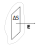
\includegraphics{electrode.pdf}}
	\caption{Элемент поверхности произвольного электрода}
	\label{fig:electode}
\end{figure}

Вероятность возникновения стримера с элемента площади $\Delta S$ за малое время $\Delta t$ можно записать, как
\begin{equation}
	P_s(E_n, \Delta S, \Delta t) = f(E_n)\Delta S \Delta t
	\label{eq:prob-deltas}
\end{equation}
где $E_n$ "--- нормальная компонента электрического поля, $f(E_n)$ "--- зависящая от поля вероятность возникновения стримера в единицу времени на единицу площади поверхности проводника. Функция $f(E_n)$ определяется составом газовой среды. Для стримерного разряда в воздухе функция $f(E_n)$ зависит от направления электрического поля на поверхности электрода. Таким образом, модель учитывает асимметрию критических полей развития стримеров положительной и отрицательной полярностей, причем отрицательные стримеры, в соответствии с многочисленным экспериментам \cite{Bazelyan1997}, имеют вдвое большие критические поля. Заметим, что $f(E_n)$ не является плотностью веротяности и поэтому не нормирована на единицу. Её физический смысл "--- количество возникающих стримерных разрядов на~$1\,\text{м}^2$ за 1~с при заданном поле $E_n$.

Выражение~\eqref{eq:prob-deltas} может быть записано в виде дифференциалов:
\begin{equation}
	dp_s(E_n) = f(E_n)dS dt
	\label{eq:prob-diff}
\end{equation}

В рамках рассматриваемой модели роль электродов, дающих начало пучкам стримеров, то есть новым ребрам и вершинам графа, играют идеально проводящие сферы, расположенные в вершинах графа. Распределение электрического поля на поверхности сферы во внешнем поле $\vec E_0$ описывается следующим выражением:
\begin{equation}
	E_n(\theta) = 3|\vec E_0 | \cos \theta + E_1 ,
	\label{eq:e-on-sphere}
\end{equation}
где $\vec E_0$ "--- внешнее по отношению к рассматриваемой сфере поле, создаваемое постоянным вертикальным полем $E_{ext}$ и зарядами, сосредоточенными на всех прочих вершинах графа, $\theta$ "--- угловая координата точки на сфере относительно направления внешнего поля $\vec E_0$, $E_1$ "--- собственное поле сферы, которое при величине ее заряда $q_i$ и радиусе $R$ может быть найдено как
\begin{equation}
	E_1 = \kelec \frac{q_i}{R}.
\end{equation}

Используя \eqref{eq:prob-diff} и \eqref{eq:e-on-sphere} для любого малого промежутка времени $dt$ можно сгенерировать случайное событие <<возникновение стримера>> методом Монте-Карло. Более подробно принцип генерации этого события рассмотрен в разделе \ref{sec:streamer-generation}. В качестве расстояния, на которое новая вершина удалена от уже имеющейся, принимается константа $L_0$, одинаковая для всей модели. Величина $L_0$ выбирается достаточно маленькой, чтобы между ветвлениями стримера успевало возникнуть несколько не ветвящихся участков.

Отметим, что узлы динамического графа могут располагаться сколь угодно близко друг к другу. Направление ветвления моделируемых проводников определяется методом Монте-Карло из полного диапазона телесных углов, равного $4\pi$ стерадиан. Степень ветвления вершины ограничивается лишь локальным значением электрического поля, то есть один и то же узел, в принципе, может быть источником для неограниченного числа рёбер. Для сравнения, в случае моделей, использующих пространственную решетку, число соседних узлов и, следовательно, возникающих из одной вершины связей, всегда конечно и ограничено числом 26. Таким образом, в данной модели структура проводников и их связность может быть гораздо более богатой, чем в случае моделей, использующих пространственные решетки.

\highlight{Бифуркация типа \ref{emun:bif-connect}.} Параметризация процесса образования новой связи между уже имеющимися узлами $i$ и $j$ системы происходит при выполнении следующих условий:
\begin{enumerate}
	\item Величина среднего поля между вершинами больше пороговой:
	\begin{equation}
		\frac{|\varphi_i - \varphi_j|}{L_{i,j}} > E^*
		\label{eq:conn-condition-1}
	\end{equation}
	где $L_{i,j}$ "--- расстояние между вершинами, $E^*$ "--- пороговое поле
	\item Вершины расположены достаточно близко:
	\begin{equation}
		L_{i,j} > \xi L_0
		\label{eq:conn-condition-2}
	\end{equation}
	где $\xi$ "--- коэффициент порядка $1\ldots10$.
\end{enumerate}
В расчётах величина порогового поля $E^*$ принимается равной $3\cdot10^5\,\text{В}/\text{м}$, коэффициент $\xi = 3$.

\highlight{Бифуркация типа \ref{emun:bif-remove}.} Отмирание ребра графа $k$ происходит при падении его проводимости, определяемой \eqref{eq:ioi-param}, ниже критического значения. Условие удаления ребра выглядит следующим образом:
\begin{equation}
	G_k < \lambda G_0
\end{equation}
где~$G_0$ "--- начальная проводимость ребра, а~$\lambda$ "--- коэффициент принимаемый в расчётах равным 0,95. Из 	\eqref{eq:temp-evo} и \eqref{eq:ioi-param} следует, что ребро, в котором развилась ионизационно-перегревная неустойчивость, не может исчезнуть.

При отмирании проводящего ребра графа одна или несколько вершин могут оказаться отсоединены от основного канала разряда. Впоследствии они могут снова оказаться <<подключенными>> к разрядной структуре при выполнении \eqref{eq:conn-condition-1} и \eqref{eq:conn-condition-2}, либо же оставаться изолированными, внося вклад в пространственный заряд. Диссипация заряда за время моделирования (порядка 1-2\,мс) считается пренебрежимо малой. За счёт наличия изолированных вершин, окружающих разрядный канал, модель воспроизводит чехол лидера.

\subsection{Генерация события возникновения узлов модельного графа}
\label{sec:streamer-generation}
Рассмотрим более подробно вопрос генерации случайного события возникновения нового пучка стримеров. Процесс пробоя воздуха параметризуется некоторой функцией $f(E)$ согласно формуле \eqref{eq:prob-diff}. При этом, согласно \eqref{eq:e-on-sphere}, электрическое поле на поверхности сферы можно записать, как 
\begin{equation}
	E_n(\theta) = 3E_0 \cos \theta + E_1,
\end{equation}
где $E_0$ "--- внешнее поле, вдоль положительного направления которого направлена ось $\theta = 0$, а $E_1$ "--- собственное поле вершины сферической вершины графа. Запишем \eqref{eq:prob-diff} с учётом симметрии:
\begin{equation}
	dp(\theta) = 2\pi R^2 f(E(\theta)) \sin \theta d\theta
\end{equation}
произведя замену переменных $\xi = \cos \theta$, получим дифференциальное распределение
\begin{equation}
	dp(\xi) = -2\pi R^2 f(3E_0 \xi + E_1) dt,
\end{equation}
откуда можно получить интегральную вероятность
\begin{equation}
	dP(\theta<\theta_0) = \frac{2\pi R^2}{3E_0} \left( F(3E_0 + E_1) - F(3E_0 \cos \theta_0 + E_1)\right)dt,
	\label{eq:total-prob}
\end{equation}
где $F(x)$ "--- неопределённый интеграл функции $f$. В обозначении $dP$ присутствует дифференциал, поскольку вероятность по-прежнему записывается для дифференциально малого промежутка времени $dt$.

Для того, чтобы при конкретном $dt$ сгенерировать случайное событие, вероятность которого определяется выражением \eqref{eq:total-prob}, необходимо сгенерировать случайную величину $\zeta$ из интервала $[0, 1)$. Максимальное значение $dP$ достигается при $\theta = \pi$:
\begin{equation}
	dP_{max}(\theta<\theta_0) = \frac{2\pi R^2}{3E_0} \left( F(3E_0 + E_1) - F(-3E_0 + E_1)\right)dt,
	\label{eq:total-prob-max}
\end{equation}
В случае, если $\zeta > dP_{max}$, за выбранный интервал времени $dt$ событие не происходит. В противоположном случае, новый сегмент стримера возникает, и его направление $\theta$ определяется корнем уравнения
\begin{equation}
	F(3E_0 \cos \theta + E_1) =  F(3E_0 + E_1) - \zeta \frac{3E_0}{2\pi R^2 dt},
	\label{eq:theta-equation}
\end{equation}

В силу симметрии задачи, при возникновения нового сегмента стримера, его угловое направление $\varphi$ генерируется из равномерного распределения по интервалу $[0, 2\pi)$.

Разработанный подход к генерации события применим для произвольной функции $f(E)$ при условии численного решения уравнения \eqref{eq:theta-equation}. Поскольку $F = \int f dE$ "--- монотонна, применимы стандартные методы решения алгебраического уравнения, например "--- серединное деление. Для оптимизации расчётов, функцию $F$ нужно однократно табулировать.

Использованные в расчётах парметры приведены в таблице~\ref{tab:parameters}.
\begin{table}[h]
	\caption{Расчётные параметры модели}
	\label{tab:parameters}
	\begin{center}
		\begin{tabular}{l|l}
			Параметр & Значение \\
			\hline
			Внешнее электрическое поле, $E_{ext}$ & $2,7\cdot 10^{5}\,\text{В}/\text{м}$ \\
			Радиус вершины, $R$ & 3\,см \\
			Радиус ребра, $r$ & 1,4\,мм \\
			Длина ребра, $l$ & 30\,см \\
			Плотность воздуха, $\rho$ & $0,63\,\text{кг}/\text{м}^3$ \\
			Удельная теплоемкость воздуха, $c$ & $10^3\,\text{Дж}/(\text{кг}\cdot\text{К})$ \\
			Начальная проводимость ребра, $G_0$ & $1\cdot10^{-10}\,\text{См}/\text{м}$ \\
			Постоянная роста проводимости, $\eta$ & $4.3\cdot10^{-5}\,(\text{В}/\text{м})^{-2}\text{с}^{-1}$ \\
			Постоянная релаксации проводимости, $\beta$ & $2,5\cdot10^6\,\text{с}^{-1}$ \\
			Пороговая температура перегревной неустойчивости, $T^*$ & $3000\,\text{К}$ \\
			%Порог гашения тока, $\lambda$ & 0,95 \\
			Пороговое поле инициации положительных стримеров, $E^+$ & $0.5\cdot 10^{6}\,\text{В}/\text{м}$\\
			Пороговое поле инициации отрицательных стримеров, $E^-$ & $1.0\cdot 10^{6}\,\text{В}/\text{м}$\\
		\end{tabular}
	\end{center}
\end{table}

\section{Результаты моделирования}
\label{sec:model-results}
В данной главе представленная транспортная самоорганизующаяся модель развития искрового разряда в воздухе была применена к изучению процесса инициации лидера молнии.
\begin{figure}[h]
	\center{\includegraphics[width=0.8\linewidth]{model-pre-leader.png}}
	\caption{Визуализация долидерной стадии развития модельного разряда. Возникновение первых одиночных стимеров, их объединение в связную токовую структуру и появление первых отрицательных стримеров.}
	\label{fig:pre-leader}
\end{figure}

\begin{figure}[h]
	\center{\includegraphics[width=0.8\linewidth]{model-leader-composition.png}}
	\caption{Визуализация лидерной стадии развития молниевого разряда. Распространение биполярного лидера молнии.}
	\label{fig:model-leader-composition}
\end{figure}
На \figRef{fig:pre-leader} показана временная динамика моделирования долидерной части процесса зарождения молниевого канала в облаке. Спустя~$t=100$\,мкс от начала моделирования система состоит всего из 22-х вершин с небольшим количеством перманентно возникающих и гаснущих связей. Электрическое поле, создаваемое разделёнными зарядами, на данном этапе недостаточно для возникновения большего числа стримерных каналов. Через~500\,мкс от начала моделирования количество узлов составляет~3330. Разряд на данном этапе представляет собой совокупность слабо связанных проводников, образующих группы по 2-3~ребра, причем большинство связей гаснет через 10-20\,мкс после появления. Затем число рёбер начинает ускоренно расти, и в момент времени $t = 800$\,мкс наблюдаются устойчивые цепочки связанных проводников, эффективно прогреваемых токами поляризации. При этом общее число узлов модели составляет~25\,тысяч. Электрическое поле на нижнем конце разряда становится достаточным для возникновения отрицательных стримеров.

На \figRef{fig:model-leader-composition} приведена временная динамика моделируемого молниевого канала после возникновения стримерно-лидерного перехода. В верхней части рисунка показаны проводящие структуры, в нижней "--- распределение заряда в пространстве. Начиная с момента времени $t = 927$\,мкс биполярный лидер стремительно развивается двунаправленным образом: его положительная часть распространяется вверх, а отрицательная "--- вниз, причем головки обоих лидеров продвигаются с примерно одинаковой скоростью порядка 210 км/с. К моменту времени $t = 1116$\,мкс число вершин модельного графа возрастает до 484\,тысяч.

На \figRef{fig:model-leader-positive-end} показаны структура проводников и распределение заряда на конце положительной части биполярного лидера молнии в момент времени $t = 1116$\,мкс. Для простоты восприятия на данном рисунке отсутствуют холодные стримерные каналы и узлы, имеющие близкий к нулю заряд.

\begin{figure}[h]
	\center{\includegraphics[width=0.8\linewidth]{midel-positive-end.png}}
	\caption{Увеличенный фрагмент  конца положительной часи лидерного канала, визуализирующий структуру проводящих связей и распределение пространственного заряда в момент времени $t = 1116$\,мкс от начала моделирования.}
	\label{fig:model-leader-positive-end}
\end{figure}

\begin{figure}[h]
	\center{\includegraphics[width=0.8\linewidth]{currents.png}}
	\caption{Осциллограмма тока в канале зарождающегося лидера молнии.}
	\label{fig:full-current-vs-time}
\end{figure}

На \figRef{fig:full-current-vs-time} приведена осциллограмма тока в канале зарождающегося лидера молнии. График приведён с момента времени $t = 500$\,мкс, поскольку до этого отдельные пучки стримеров не образуют связанную цепочку. Начиная с $t = 500$\,мкс, по мере развития коллективного канала ток стабилизируется и постепенно растёт. Увеличение тока на порядок в момент времени $t = 927$\,мкс соответствует сримерно-лидерному переходу "--- возникновению молниевого лидера. Второй, более плавный скачёк тока при $t = 1100$\,мкс соответствует моменту соединения двух ветвей положительной части лидера с образованием петли, что привело к снижению общего сопротивления канала.

\section{Обсуждение результатов моделирования}
\label{sec:model-talks}
Разряд начинает развиваться из простейшей проводящей структуры, образованной парой изначально незаряженных вершин и ребром между ними, поляризация которой происходит под действием внешнего электрического поля. Основываясь на идеях, изложенных в работах \cite{Iudin2017}, \cite{todo}, можно ассоциировать такую пару вершин с дипольной областью повышенной проводимости с верхним положительным и нижним отрицательным полюсами. В работе \cite{todo} показано, что поляризация дециметровых ионных областей повышенной проводимости в поле грозового облака обеспечивает необходимый для начала роста положительных стримеров уровень усиления электрического поля на ее концах.

Стоит отметить, что электрические параметры модельного лидера ставят его в промежуточное положение между лабораторной длинной искрой и <<зрелым>> лидером молнии. Так, проводимость лидерного канала, составляющая порядка 10\,См/м (предельно возможное в модели значение), превышает типичную проводимость лабораторного положительного лидера, равную 1\,См/м \cite{Raizer2009}, но на три порядка меньше проводимости дугового разряда молнии (порядка  $10^4 \text{См}/\text{м}$ \cite{RakovUman2005}). То же самое можно сказать о токе лидерного канала, составляющем порядка 10\,А (см.~рисунок~\ref{fig:full-current-vs-time}), в то время как типичные токи в каналах лабораторного и молниевого лидеров равны 1\,А\,\cite{Raizer2009} и 100\,А\,\cite{RakovUman2005} соответственно. Продольное поле модельного лидерного канала падает до $2.1\cdot 10^5\,\text{В}/\text{м}$, что значительно меньше поля в канале только что сформировавшегося стримера, которое, по крайней мере, должно превышать порог инициации (5~и~10\,кВ/см для положительных и отрицательных стримеров соответственно).  Погонная плотность чехла заряда, составляющая 40\,мкКл/м и 60\,мкКл/м для положительного и отрицательного модельных лидеров соответственно, также оказывается меньше соответствующей величины для лидера молнии, по некоторым оценкам составляющей 700-1000\,мкКл/м \cite{RakovUman2005}.

Приведенные характеристики модельного лидера выглядят вполне естественно, так как в данной работе мы воспроизводим процесс формирования лидера молнии в облаке, то есть рассматриваем переходную стадию от стримерной формы разряда к лидерной. Разумно предположить, что на начальном этапе развития электрические свойства <<молодого>> канала лидера молнии будут переходными между слаботочными лабораторными искровыми разрядами и установившимся дуговым каналом развитой молнии. В этом плане присутствующее в модели ограничение на максимально допустимую проводимость канала, равную 10\,См/м, не сказывается негативно на корректности результатов моделирования.

Отметим, что в данной работе впервые, насколько известно авторам, учтена асимметрия полей распространения положительных и отрицательных стримеров (см. таблицу \ref{tab:parameters}), необходимость чего подчеркивается в работе \cite{VanderVelde2013}. Введение вдвое большего порогового поля роста отрицательных стримеров по сравнению с положительными позволило в полной мере воспроизвести процесс, описанный в работе \cite{Griffiths1976}, в которой подчеркивается ведущая роль именно положительных стримеров. Так, в модели сначала появляются положительные стримеры, переносящие положительный заряд в направлении роста и коллективным образом аккумулирующие отрицательный заряд в области точки-источника пучка. При этом создаваемое отрицательным зарядом поле позволяет инициировать отрицательные стримеры, возникающие к моменту времени $t = 800$\,мкс (см. рис. \ref{fig:pre-leader}). Используемые в работе пороговые поля роста положительных и отрицательных стримеров, равные 5~и~10\,кВ/м соответственно, совпадают со средними полями в стримерных зонах положительного и отрицательного лидеров при нормальных условиях соответственно \cite{Bazelyan1997}. Поскольку развитие модельного разряда происходит на высоте 6-и км над уровнем моря, рассматриваемые поля, в соответствии с хорошо известным законом $E/p=const$, должны быть меньше. Известно, однако, что используемые в численных моделях развития разрядов пороговые поля определяются пространственным разрешением модели, поэтому их следует рассматривать как некие эффективные значения. Для беспрецедентно малой длины элемента разрядного канала~30\,см, рассматриваемой в модели, используемые пороговые поля роста положительных и отрицательных стримеров приводят к адекватному описанию процесса инициации молниевого канала в облаке.   

Одним из важнейших свойств представленной модели является включение в неё процесса стримерно-лидерного перехода, без которого описание зарождения молниевого лидера было бы невозможным. В рамках модели преобразование стримерного канала в лидерный описывается соотношениями \eqref{eq:temp-evo} -- \eqref{eq:alph-param}, параметризующими процесс ионизационно-перегревной неустойчивости (см., например, \cite{Raizer2009}). Рост температуры газа за счет джоулева энерговыделения $\sigma E^2$ (см. соотношение \eqref{eq:temp-evo}) в пучке однонаправленных стримеров, с которым мы ассоциируем модельную связь, приводит к увеличению приведенного поля $E / N$ вследствие падения концентрации частиц $N$, что, в свою очередь, обеспечивает резкий рост температуры электронов $T_e$. В силу резкой зависимости частоты ионизации от $T_e$ повышение температуры приводит к сильному возрастанию концентрации электронов и дальнейшему увеличению проводимости канала. Критерием, по которому в модели стримерные каналы отделяются от лидерных, является температура канала. При превышении температурой канала порогового значения $T^* = 3000\,K$, происходит быстрый рост его проводимости (см. выражение \eqref{eq:ioi-param}), а сам канал из стримерного превращается в лидерный. Выбор пограничной температуры $T^*$, отделяющей стримерное состояние канала от лидерного, на уровне $3000\,K$ связано с тем, что для сохранения электронной проводимости канал должен быть нагрет хотя бы до нескольких тысяч градусов \cite{Bazelyan1997}. Рассмотрение именно температуры в качестве основного фактора, определяющего состояние канала, соответствует концепции ионизационно-перегревной неустойчивости, наиболее медленным звеном которой является нагревание газа \cite{Raizer2009}.

Реализованная в модели концепция, при которой коллективное действие множества положительных стримеров, создавая разделение заряда в относительно малой области пространства, локально изменяет свойства диэлектрической среды и подготавливает условия для формирования канала лидера молнии, находит ряд экспериментальных подтверждений. Так, в работах \cite{Rison2016, Chapman2017}, на основе анализа данных натурных измерений делается вывод о том, что появлению молнии предшествует стадия изменения электрического поля, причем в работе \cite{Rison2016} утверждается, что данные изменения создаются так называемым быстрым пробоем на положительных стримерах (fast positive breakdown). Данный тип пробоя является чисто диэлектрическим, то есть не приводит к формированию лидерного канала, и обеспечивается интенсивным развитием системы положительных стримеров, происходящем на масштабах порядка 100-500 м за времена порядка 10 мкс, что соответствует эффективной скорости распространения разряда, лежащей в диапазоне $10^7 - 10^8 \text{м}/\text{с}$.

Представленная в данной работе транспортная самоорганизующаяся модель инициации молнии в облаке корректно воспроизводит ряд коллективных эффектов, явным образом не заложенных в исходный алгоритм. Во-первых, модель детально воспроизводит процесс образования чехла лидерного канала, являющегося источником импульса тока молнии на наиболее мощной по энергетике стадии возвратного удара. В данной работе образование чехла является естественным элементом модели и обеспечивается отмиранием слаботочных разрядных каналов. Хотя принято выделять два возможных источника чехла заряда лидерного канала: стримерная зона лидера и возникающая с боковой поверхности канала стримерная корона \cite{Maslowski2006}, в данной работе можно говорить только о первом механизме, так как используемый в модели 5-и сантиметровый радиус узла, с которого возникают модельные разряды, не позволяет адекватно описывать электрическое поле на поверхности лидерного канала, имеющего радиус порядка долей миллиметра \cite{BazelyanRaizer-FizikaMolniiIMolniezaschity}. Во-вторых, скорости распространения положительной и отрицательной частей модельного разряда на стадии лидера примерно совпадают и составляют около 210\,км/с, что хорошо согласуется с данными натурных наблюдений \cite{VanderVelde2013}. 

Из рисунков \ref{fig:model-leader-composition} и \ref{fig:model-leader-positive-end} видно, что каналы положительной и отрицательной частей биполярного лидера окружены отрицательным и положительным цилиндрическими слоями заряда соответственно. Подобный эффект наблюдался в модели \cite{Luque2014}, посвященной изучению коллективной динамики растущей с плоского электрода системы положительных стримеров. Авторы объясняют накопление отрицательного заряда в области основания положительной стримерной системы недостаточной проводимостью примыкающих к аноду разрядных каналов: поступающий от внешней более разветвленной части системы положительных стримеров отрицательный заряд <<застревает>>, не доходя до электрода, из-за низкой транспортной способности каналов внутренней части разрядного древа. Можно предположить, что и в нашем случае наличие примыкающих к поверхностям лидерных каналов слоев заряда, знак которых противоположен полярностям окруженных ими каналов, объясняется тем, что проводимость ближайших к лидерным каналам стримеров оказывается недостаточной для того, чтобы полностью поставлять к лидерам приходящий от разветвленной системы внешних стримеров заряд. Заметим, что в той же работе обосновывается физичность процесса установления проводящих связей между разрядными каналами одной и той же стримерной системы, возникающих, если заряды в паре близко расположенных узлов разрядной структуры в процессе развития разряда приобретают разные знаки. В нашей модели процесс возникновения ребер между парой уже существующих вершин происходит аналогичным образом (см. раздел \ref{sect:bifurcations}).

\section{Технические аспекты модели}
\label{sec:model-tech}
Для численного расчёта транспортной самоорганизующейся модели был разработан специальный программный пакет, в основе которого лежит принцип модульности: логическая структура транспортной системы, законы эволюции динамических переменных и возникновения бифуркаций, разностная схема, подсистема вывода и прочие компоненты независимы друг от друга. Такой подход позволяет при необходимости лёгко модифицировать физические принципы, лежащие в основе модели.

\subsection{Алгоритм}
Моделирование процесса инициации молнии происходит с автоматическим выбором шага по времени $\Delta t$. Расчёты в рамках одной итерации модели упрощённо описываются следующим образом:
\begin{enumerate}
	\item Интегрирование динамических переменных, привязанных к вершинам и рёбрам графа, по схеме Рунге-Кутты четвёртого порядка с текущим шагом по времени~$\Delta t$ \label{enum:rk-iter}
	\begin{enumerate}
		\item Вычисление электрических полей и потенциалов во всех вершинах графа \label{enum:sec-val}
		\item Вычисление правых частей дифференциальных уравнений для всех динамических переменных для подшага метода Рунге-Кутты
		\item Выполнение подшага \label{enum:substep}
		\item Выполнение п.\,\ref{enum:sec-val} -- п.\,\ref{enum:substep} для всех подшагов
		\item Оценка приращений динамических переменных. Модификация шага по времени $\Delta t$ при недостаточной или избыточной точности расчёта. В случае, если шаг необходимо уменьшить "--- повторный расчёт итерации начиная с п.\,\ref{enum:rk-iter}
	\end{enumerate}
	\item Расчёт вероятностей и параметров бифуркаций системы в соответствии с введёнными правилами:
	\begin{enumerate}
		\item Генерация новых вершин и рёбер графа методом Монте-Карло в соответствии с \eqref{eq:total-prob-max}, \eqref{eq:theta-equation}
		\item Поиск и удаление рёбер с проводимостью ниже порогового значения
		\item Нахождение и соединение пар вершин, среднее поле между которыми превосходит критическое
	\end{enumerate}
	\item Вывод текущего состояния модели в файлы, если прошло достаточно модельного времени от предыдущего сохранения состояния, визуализация через графические интерфейс, если требуется.
\end{enumerate}

\subsection{Оптимизация расчёта электрического поля}
Наиболее затратной с точки зрения процессорного времени задачей является расчёт суммарного электрического поля в каждой вершине графа, порождаемого каждой другой вершиной графа (п.~\ref{enum:sec-val}). Расчёт с прямым суммированием полей по формуле \eqref{eq:coulomb} имеет сложность $O(N^2)$ на каждой временной итерации, где $N$~"---~число вершин графа. Такая сложность привозит к сильному замедлению расчётов в процессе распространения лидера, когда за каждую единицу времени добавляется приблизительно одинаковое количество вершин. В таком случае соотношение между модельным временем и временем вычислений принимает вид
\begin{equation}
	t_\text{мод} \propto t_\text{выч}^{1/3}.
\end{equation}

Для оптимизации расчётов кулоновского поля реализовано восьмеричное дерево "--- случай k-дерева \cite{Bentley1975} для трёхмерного пространства. Идея алгоритма состоит в следующем: все вершины графа можно ограничить снаружи кубом некоторого размера. Такой куб можно разделить на 8~подкубов с вдвое меньшей стороной. Каждый из них разделить ещё на 8~подкубов и т.\,д. до тех пор, пока в подкубе не останется только одна вершина графа. Пустые подкубы отбрасываются. Таким образом можно построить восьмеричное дерево, листьями которого будут вершины графа, и каждому узлу которого будет соответствовать определенный куб в пространстве (\figRef{fig:octree}). За время порядка $O(N\log_8 N)$ можно построить такое дерево, а также определить для каждого куба положение <<центра масс>> положительного и отрицательного зарядов и их величины.
\begin{figure}[h]
	\center{\includegraphics[width=0.8\linewidth]{octree.png}}
	\caption{Восьмеричное разбиение пространства}
	\label{fig:octree}
\end{figure}

Когда восьмеричное дерево построено, можно за время порядка $O(\log_8 N)$ находить вершину, ближайшую к любой заданной точке, а также эффективно рассчитывать электрическое поле. Для приблизительного расчёта поля от вершин, расположенных в достаточно далёком кубе, можно вычислить поле центра масс данного куба. При этом зависимость приемлемого размера такого <<куба~усреднения>> от расстояния до точки, в которой вычисляется поле, может быть задана произвольно. Таким образом алгоритм позволяет произвольно регулировать соотношение между скоростью и точностью вычислений. Время расчёта электрического поля во всех вершинах графа становится существенно меньше, чем $O(N^2)$.

\subsection{Программный код}
Программный пакет написан на языке C++ в соответствии с принципами объектно-ориентированного программирования. На текущий момент пакет состоит из, приблизительно, 15 тыс. строк кода. В разработке применяются следующие технологии и библиотеки:
\begin{itemize}
	\item \textbf{Параллелизация вычислений} выполняется при помощи библиотеки Intel TBB.
	\item \textbf{Вывод} состояния графа в файлы в формате VTK осуществляется при помощи библиотеки libVTK
	\item \textbf{Визуализация данных} в реальном времени реализована при помощи Qt и libVTK
	\item \textbf{Модульное тестирование} различных компонентов системы работает на основе библиотеки GTest
	\item \textbf{Прочие вспомогательные задачи} "--- разбор конфигурационных файлов, работа с командной строкой и т.п. осуществляются при помощи компонентов библиотеки Boost
	\item \textbf{Визуализация готовых расчётов,} генерация видео и оформление изображений для публикаций производится внешней программой ParaView.
\end{itemize}

Для большинства расчётов использовался сервер с двумя процессорами Intel Xeon E5-2660 @ 2.60GHz с общим количествов физических ядер 20\,шт., 128\,Гб ОЗУ (однако задаче требуется всего лишь 1-2\,Гб).

\section{Выводы}
Разработана транспортная самоорганизующаяся модель процесса инициации молнии, описывающая процессы от образования областей спонтанной проводимости до распространения и ветвления билидера. Разработан специализированный программный пакет для проведения расчётов модели. Продолжительность моделируемых процессов составляет порядка 1\,мс, пространственный масштаб проводящих структур "--- около 100\,м.

Модель обладает рядом уникальных особенностей: отсутствие пространственной сетки, неограниченная степень ветвления, учёт асимметрии возникновения положительных и отрицательных стримеров, самосогласованное моделирование стримерно-лидерного перехода при помощи параметризации ионизационно-перегревной неустойчивости.

Модель воспроизводит реалистичные макроскопические параметры разряда, такие, как ток в канале билидера, погонный заряд чехла лидера, скорость распространения лидера, поле в его канале. Воспроизводимая картина развития разряда соответствует экспериментальным наблюдениям. Таким образом, при помощи модели показано, что одного лишь механизма индукционного разделения заряда достаточно для возникновения билидера в докритическом поле облака при условии возникновения областей проводимости порядка~10-30\,см.

\FloatBarrier
